\documentclass[12pt,oneside]{book}
\pagestyle{headings}

% Note that the line below could be modified to suit a
% particular system since the "geometry" package behaves
% differently in Unix, Windows and Mac, especially for the
% top margins.
% Adjust the parameter "top" (measuring the height of the
% space allocated to a header) and "headsep" (measuring
% the distance from the bottom of the header to the
% first line of text.
\usepackage[top=1.3in,left=1.5in,bottom=1in,right=1in,headsep=0.5in]{geometry}

\usepackage{setspace}
\onehalfspacing
%\doublespacing

% Headers and footers for thesis
\usepackage{fancyhdr}

\markboth{}{}
\newcommand\startchapter[1]{\chapter{#1}\thispagestyle{myheadings}}
\newcommand\startappendix[1]{\chapter{#1}\thispagestyle{myheadings}}
\newcommand\startfirstchapter[1]{\chapter{#1}}

% Manual addition of section to Table of Contents
\newcommand\TOCadd[1]{\newpage\phantomsection\addcontentsline{toc}{chapter}{#1}}

% Float Customization
\renewcommand{\floatpagefraction}{0.01}

% Customization of Tables of Contents and List of Figures/Tables
\usepackage{tocloft}
\renewcommand\cfttabpresnum{Table\ }
\renewcommand\cfttabnumwidth{0.75in}
\renewcommand\cftfigpresnum{Figure\ }
\renewcommand\cftfignumwidth{0.80in}
\newcommand{\HRule}{\rule{\linewidth}{0.5mm}}


% Long Table and decimal aligned columns
\usepackage{dcolumn}
\usepackage{longtable}

% Mathematics support
\usepackage{amsmath}
\delimitershortfall-1sp
\newcommand\abs[1]{\left|#1\right|}

\usepackage{amsthm}
\usepackage{amssymb}


% Text Control
\usepackage{xspace}
\usepackage{textcase}

% Graphics
\usepackage{wasysym}
\usepackage{graphics}
\usepackage{graphicx}   % A package to allow insertion of
                        % external image files
\graphicspath{{Figures/}}
\usepackage[caption=false]{subfig}
\captionsetup{belowskip=8pt,aboveskip=8pt}
\usepackage{multirow}
\newtheorem{remark}{Remark}
\usepackage{algorithmic}
\usepackage[ruled]{algorithm2e}
%\usepackage{epsfig}
\usepackage{epstopdf}
\usepackage{tikz}
%\usepackage{gantt}
\usepackage{titling,enumitem}
\usepackage{url}
\usepackage{makecell}
\usepackage{lscape}
\usepackage{cite}
\usepackage{nomencl}
\makenomenclature
\makeatletter
\def\thenomenclature{%
  \section*{\nomname}
  \if@intoc\addcontentsline{toc}{section}{\nomname}\fi%
  \nompreamble
  \list{}{%
    \labelwidth\nom@tempdim
    \leftmargin\labelwidth
    \advance\leftmargin\labelsep
    \itemsep\nomitemsep
    \let\makelabel\nomlabel}}
\makeatother


% Widecheck
\makeatletter
\DeclareRobustCommand\widecheck[1]{{\mathpalette\@widecheck{#1}}}
\def\@widecheck#1#2{%
    \setbox\z@\hbox{\m@th$#1#2$}%
    \setbox\tw@\hbox{\m@th$#1%
       \widehat{%
          \vrule\@width\z@\@height\ht\z@
          \vrule\@height\z@\@width\wd\z@}$}%
    \dp\tw@-\ht\z@
    \@tempdima\ht\z@ \advance\@tempdima2\ht\tw@ \divide\@tempdima\thr@@
    \setbox\tw@\hbox{%
       \raise\@tempdima\hbox{\scalebox{1}[-1]{\lower\@tempdima\box
\tw@}}}%
    {\ooalign{\box\tw@ \cr \box\z@}}}
\makeatother

\newcommand{\specialcell}[2][c]{%
  \begin{tabular}[#1]{@{}c@{}}#2\end{tabular}}
\makeatletter
\providecommand{\keywords}[1]{\textbf{Index terms---} #1}
\newcommand{\defeq}{\buildrel {\text{ def }}\over =}



\begin{document}
%/////////////////////////////////////////////////////////////////////////////////////////////////////////////////////
\startchapter{A Prediction Model}
\label{chap:predictionModel}
\section{Motivation}
As discussed in Chapter~\ref{chapter:introduction}, the main objective of this work is to increase the reliability of power networks in terms of power quality within given financial budget/resources. In order to monitor the power quality, power quality meters are being deployed. Since power quality meters are expensive devices, we (in chapter~\ref{chap:PQEstimation}) proposed MaxEnt based algorithm for power quality estimation on unmonitored network segments. For meter placements, we proposed conditional entropy based efficient algorithms (in chapter~{chap:meterPlacement}) that intelligently place power meters on selected network segments so that the power quality could be inferred as accurately as possible.

Since the power quality readings (exact readings from monitored links, and estimated PQ values from unmonitored links) are available now, we use these readings to estimate the state of the network and identify any potential malfunctioning device in the power network. Our objective in this chapter is to address the research challenge: \textit{how to detect a potential malfunctioning device in the power network based on available power quality readings}. In the next section, we propose an algorithm that helps to detect the malfunctioning devices in the power network.

\section{Problem Formulation}
\subsection{Assumptions}
We make below assumptions about the problem:
\begin{enumerate}
\item \textit{The transfer function or behavior $\left(f\left(d\right)\right)$ of each device $d$ in the network is known}. As discussed earlier, a device-specific power quality transfer function could be estimated through physical modeling or through the assessment of historical PQ data. In Chapter~\ref{chap:latentF}, using a real power quality dataset, we have shown how accurately an $f(d)$ could be estimated.

\item \textit{All potential malfunction devices need to be on a monitored segment.} A potential malfunction device could effectively be detected when the device itself or any of its child device is monitored in real time using a PQ meter. This assumption is realistic in the sense that if the underline link is not monitored, we cannot get the real-time status of PQ values and would not be able to detect if a device is not behaving normally. The idea is to detect if a device is significantly deviating form its normal behavior.

\item \textit{The power grid network is a tree-structured network where the electric current flows from root node to the child nodes.} Note that this is a reasonable assumption at any particular instance in time. While enterprise level power grids used in places such as hospitals and data centers often have two utility feeds available as well as an independent emergency power source, only one power source is typically used at one time. See the IEEE Gold Book~\cite{goldbook} for further information on recommended practices in the design of critical power systems.

\item \textit{The probability mass function} ($f_x\left(d_0\right)$)\textit{ of power quality values at the input link to the root node is known.} In other words, the distribution of power quality at the input to the network, usually the utility feed, is known. This is also a reasonable assumption, since electrical utilities typically report on indices such as System Average RMS Variation Frequency Index (SARFI) which is essentially a count of the number of times the magnitude and duration falls below a threshold. Furthermore, there are often independent bodies that gather statistics on power delivery service reliability that can also be incorporated into an estimate of power quality distribution~\cite{chowdhury2004reliability}.
\end{enumerate}


\begin{figure}[!t]
\centering
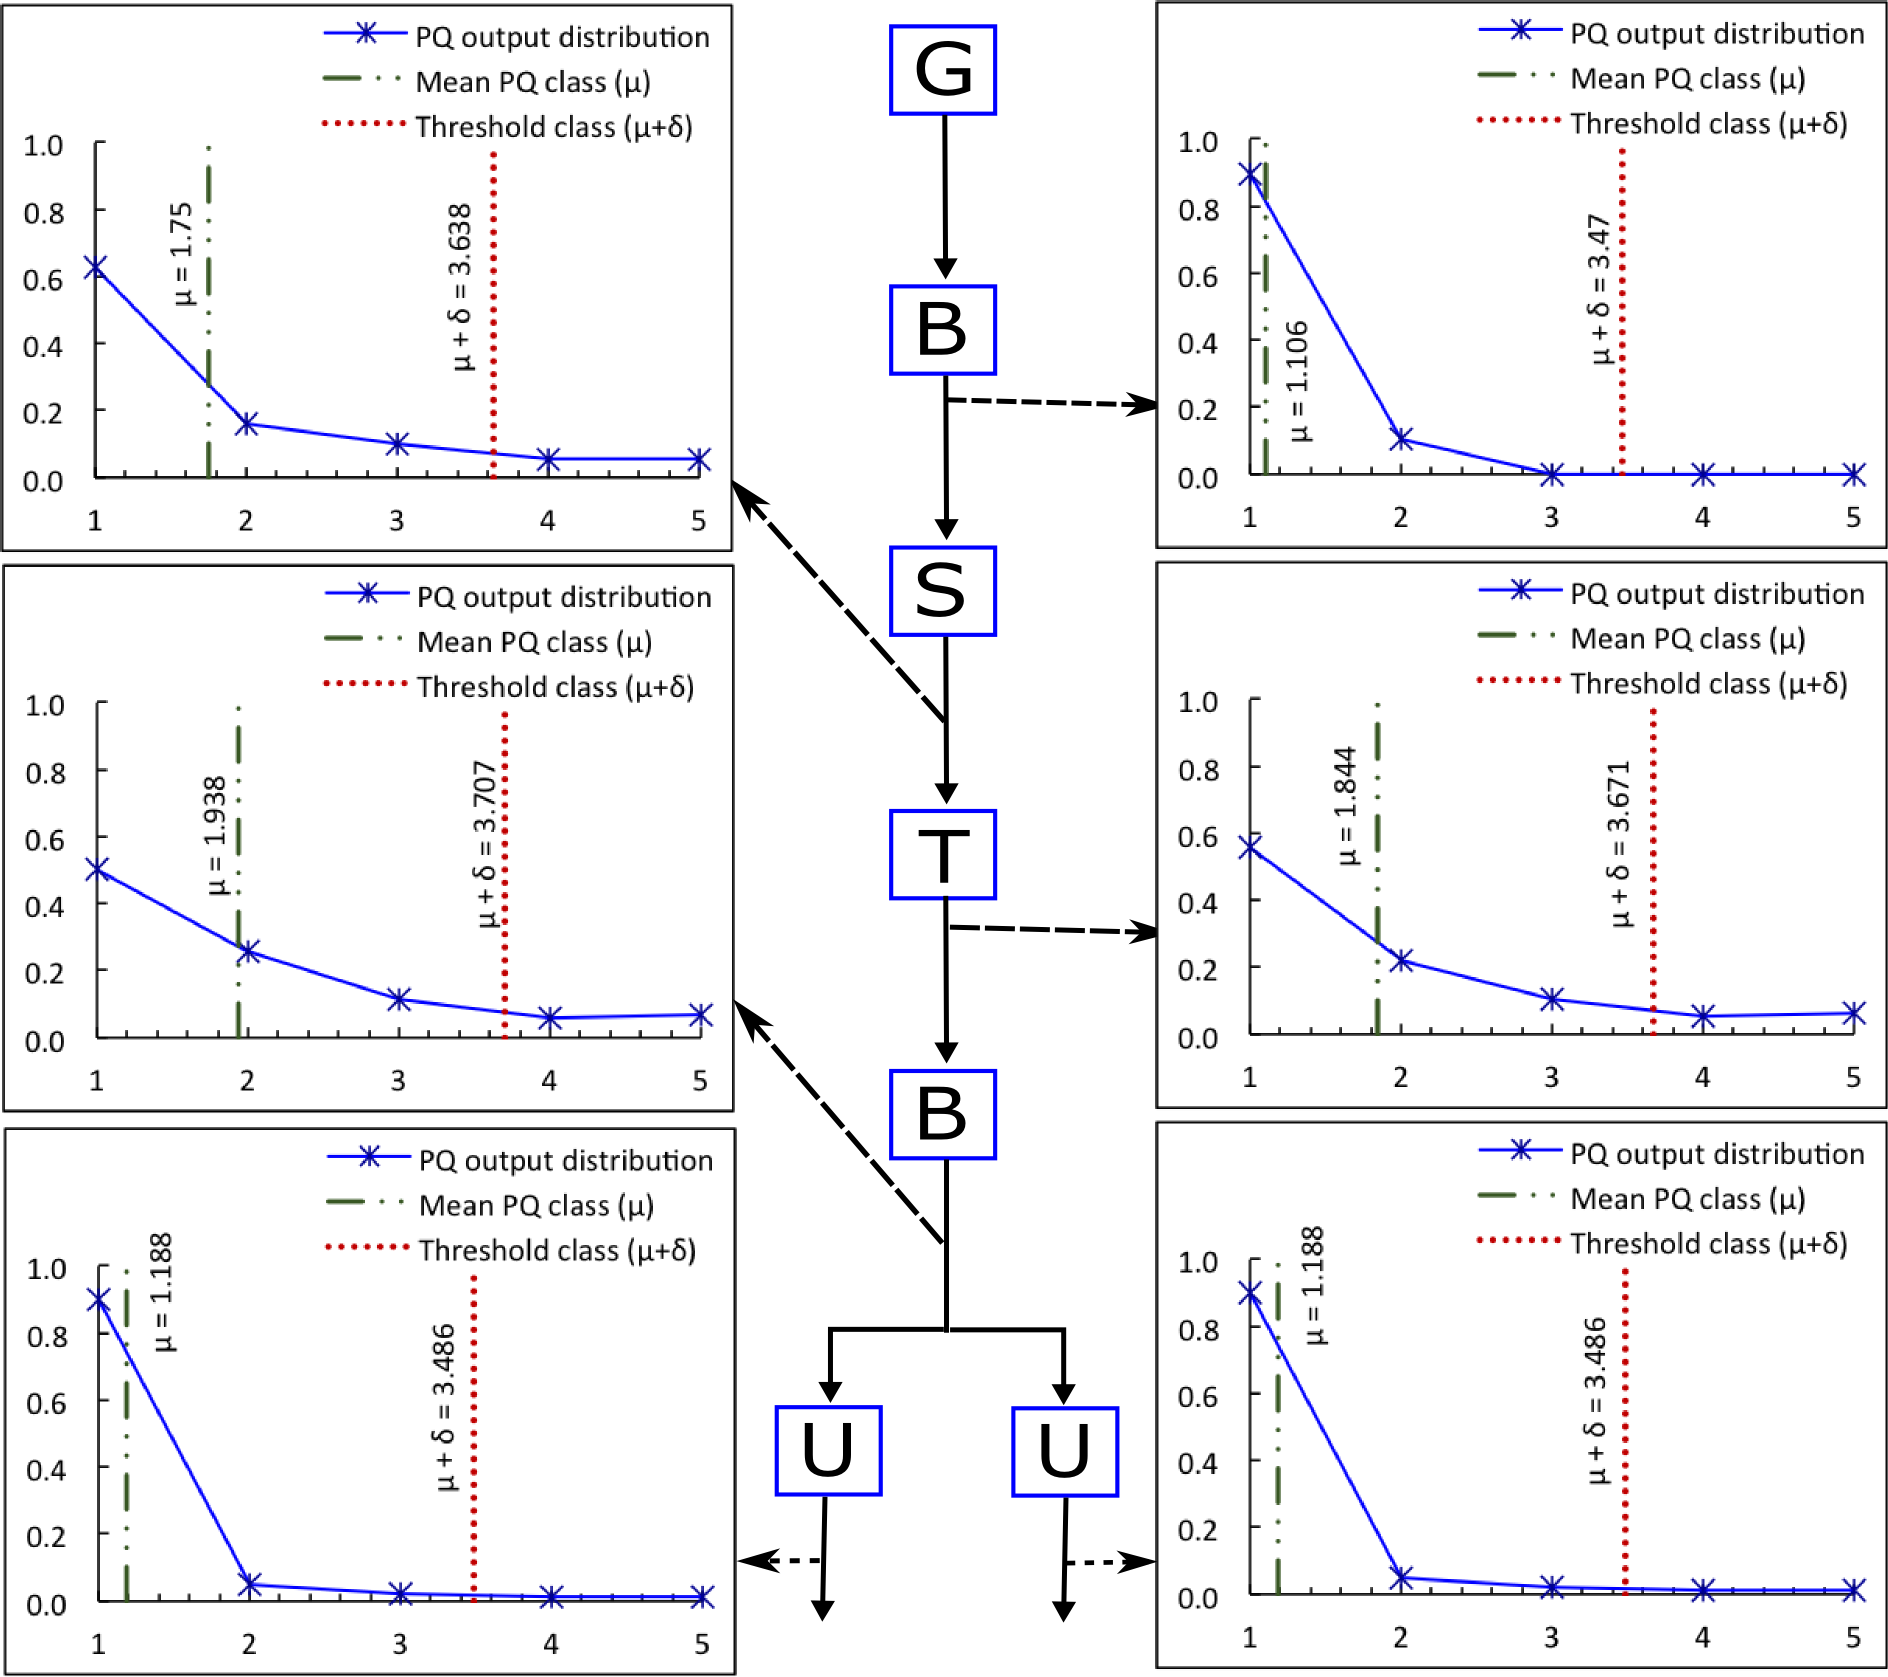
\includegraphics[width=0.98\textwidth]{PQOutputDistribution}
\caption{Power quality distributions at the output links of various devices. The average power quality class and computed threshold is shown as vertical lines in each  distribution graph. The x-axis represents the power quality class $c_i$ while the y-axis represents the probability of $c_i$. Further, the lower power quality class $c_1$ represents the best power quality while $c_5$ represents the worst power quality.}
\label{fig:outputPQDistributions}
\end{figure}

\subsection{The Problem}
We now formalize the problem of detecting a malfunction device in the network. The objective is to detect a device $d$ in the network as a malfunction device when its power quality output degrades persistently from its normal behavior. Since the transition function $f(d)$ of each device $d$ is known, we know the probability distribution of the output power quality ($f_x\left(d\right)$) at the output link of each device in the power grid network. Figure~\ref{fig:outputPQDistributions} shows the probability distributions for various devices in a sample network. The distributions are obtained/computed for the prior distribution of$\begin{array}{ccccc}[0.9947 & 0.005 & 0.0002 & 0.00009 & 0.00001]\end{array}$at the utility feed/generator.

We mathematically analyze these distributions and based on their various statistical properties, we propose out detection algorithm in next section. The proposed algorithm compares the normal behavior of a device (the $f_x\left(d\right)$) of each device with the observed behavior ($\widehat {f_x}\left(d\right)$) and compute the power quality degradation (the difference between the two distributions) as $\Delta_d$ . The objective function becomes:

\begin{equation}
\label{eq:pqPrediction}
\Delta_d = f_x\left(d\right) \defeq \widehat{f_x}\left(d\right)
\end{equation}

\noindent where the operation $\defeq$ is unknown. In the next section,  we propose algorithms to solve the equation~\ref{eq:pqPrediction}.

\section{Our Prediction Algorithms}
\subsection{A simple correlation measure}
In order to compare two probability distributions, the correlation measure is usually used where its most familiar type is the \textit{Pearson's correlation coefficient}, simply known as \textit{the correlation coefficient}. In order to use the formula, we represent the actual PQ distribution as X while the obtained distribution as Y. For the random variables X and Y, it is defined as:
\[\rho_{X,Y} = corr(X,Y) = \frac{\sum (x-\bar x) (y-\bar y)}{\sqrt{\sum (x-\bar x)^2 \sum (y-\bar y)^2}}\]

The above correlation measure could be used to compare the actual and observed PQ distributions. Generally speaking, this measure can accurately tell how much the observed distribution is similar (or different) from its actual one. When a device is perfectly behaving like its actual distribution, the measure returns a maximum value (  +1). On the other hand, when a device is producing a very different (for instance producing very bad PQ) distribution, it returns a smaller value (the smallest possible is -1). The value 0 (or closer to 0) represents that the two distribution has no correlation, i.e., they are asymmetric. Although this technique is simple to use, we found various scenarios where it is not able to accurately detect the power quality degradation. We classify the identified scenarios in two classes: 1) a malfunction device is not detected; and 2) a better PQ producing device is classified as a malfunction. Both cases are explained as follows.

\begin{figure}[!t]
\begin{centering}
\subfloat[Positive correlation ($\rho_{X,Y} = +0.95 \approx +1$)]{\label{corr_positive}
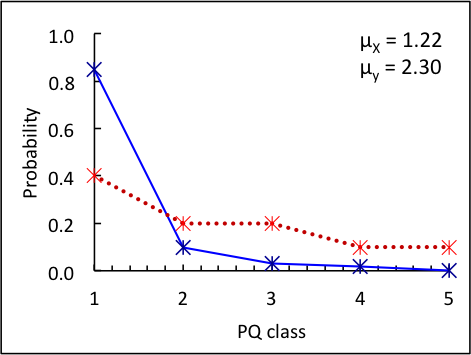
\includegraphics[width=0.48\columnwidth]{corr_positive}
}
\subfloat[Zero correlation ($\rho_{X,Y} = 0$)]{\label{corr_zero}
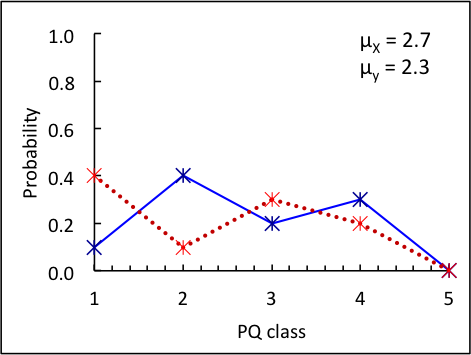
\includegraphics[width=0.48\columnwidth]{corr_zero}
}
\end{centering}

\begin{centering}
\subfloat[Negative correlation ($\rho_{X,Y} = -1$)]{\label{corr_negative_low}
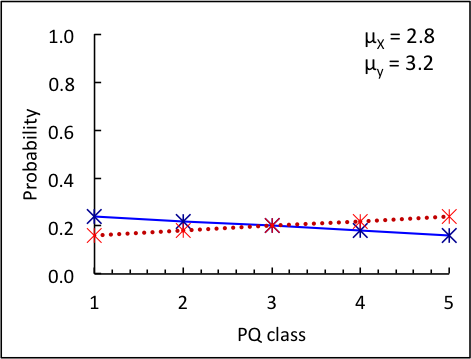
\includegraphics[width=0.48\columnwidth]{corr_negative_low}
}
\subfloat[Negative correlation ($\rho_{X,Y} = -1$)]{\label{corr_negative_high}
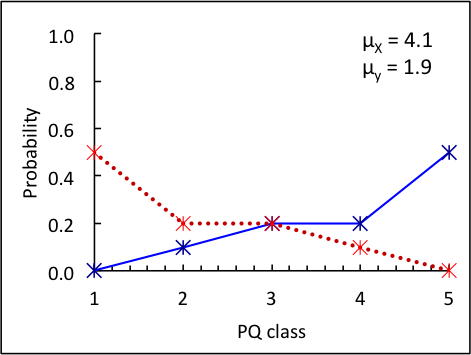
\includegraphics[width=0.485\columnwidth]{corr_negative_high}
}
\end{centering}

\caption{Various PQ distribution scenarios where the simple correlation technique is not useful.} 
\label{correlationAnalysis}
%\vspace{-0.15in}
\end{figure}

\subsubsection{Missed Detection Scenarios}
This scenario arises when a device is producing a very bad power quality (malfunctioning) and the system does not detect it. The system will classify the observed distribution as perfectly normal (similar to the normal) when the correlation is +1 (or close to +1). For all normal behaving devices, the observed distribution will be very similar to the normal and a +1 correlation will perfectly classifying them as normal. Nevertheless, we identified cases where the PQ is significantly degraded and the distributions were highly correlated. In all those cases, we cannot use the simple correlation formula. Figure~\ref{corr_positive} shows one such example where the power quality is significantly degraded and the correlation coefficient is a +1.

\subsubsection{False Detection Scenarios}
We classify a detection as false when its power quality output is similar (or slightly degraded) from its normal. Using the correlation measure, a device is detected as malfunction when the correlation coefficient is smaller (close to 0 or smaller than 0). Although we observed that this measure works in various cases, we have also been able to identify few scenarios where the simple correlation measure miss-classify devices as malfunction. These scenarios are explained in two categories as follows:

\begin{enumerate}
\item \textbf{Zero Correlation:} A zero correlation means the two distributions do not share any particular correlation. In our case, most probably, observing a distribution which do not share any correlation implies degradation in the power quality. But we cannot tell for sure if the observed distribution is good or bad. Figure~\ref{corr_zero} represents a scenario where the observed power quality is better and we can not classify the device as a malfunction simply based on a zero correlation.

\item \textbf{Negative Correlation:} In a negative correlation between two variables, the value of one variable increases while the other decreases, and vice versa. Although theoretically possible, it is rare to get a perfectly negative correlation in power quality measures. In a negative correlation, the observed distribution is either a bad or good PQ distribution than its normal. Although the probability of getting a bad PQ is higher than that of a good, it cannot always be guaranteed.

Further, although the negative correlation can quantify the symmetry of the distribution, in cannot essentially quantify how much the distribution are different. For instance, Figure~\ref{corr_negative_low} shows a perfect -1 correlation but the actual PQ degradation is very minor. Finally, for the sack of theoretical proof, Figure~\ref{corr_negative_high} demonstrate a significant PQ improvement as a power quality degradation.

\end{enumerate}


\subsection{The Average PQ class based algorithm}

for every sample -> check if f(d) varies by f1(d)\\
for the detected segment, use maxent to estimate f(d1) to f(dn)\\
sort them by descending order of variation\\
the top one is high probable.

bad power quality events\\
unit time interval\\
window size\\
an interval is bad quality interval when it is classified as >= 4\\
threshold number of bad quality intervals\\
misbehaving device on the detected link\\
candidate links are\\
use maxent


using input pdf simulation dataset was generated\\
we use f(d) as in chapter 3

If no smart meter installed on that device, need to estimate from neighboring links

- The metered link detects deviation and estimate the deviations of all devices between itself and parent metered link

\section{Evaluations}
Assume that one or more smart meters have continuously measured poor power quality. The power quality is indicated by some specific power quality index, for instance the System Average RMS Variation Frequency (SARFI) index . Based on the measured and estimated PQ values, we would like to know which device is most likely to be malfunctioning. Here, we assume that we know the transform function of each device if the device is working properly. We call these transfer functions the regular transform functions of the devices. Now, a malfunctioning device is the one whose estimated transform function deviates significantly from its regular transform function.

We plan to first give a comprehensive mathematical model of the problem. We then device a mechanism to calculate the deviation in transfer functions and finally we plan to propose an algorithm to efficiently identify any potential malfunctioning device in the power network. The proposed algorithm will be evaluated on various tree and bus structured network; specifically we will use the IEEE standard test networks for our simulations.

\section{Conclusion}
Power quality meters play an important role in the reliability of power networks. We plan to investigate the problem of identifying devices that degrade the power quality in the system. The proposed solution will be built on top of our already proposed work.


%/////////////////////////////////////////////////////////////////////////////////////////////////////////////////////
\end{document}